\chapter{Inference using nonlinear hybrid models}
\label{sec_inf_spf}
In this chapter we study the same graphical model as chapter \ref{sec_inf_lin_hybrid}, shown in figure \ref{fig_hybridmod2} for convenience, but we drop the assumption that the dynamic models used for inference are linear. The variables retain their meaning as before.     
\begin{figure}[H] 
\centering
\begin{tikzpicture}

  % Define nodes
  \node[obs] (ya) {$y_0$};
  \node[obs, right=of ya] (yb) {$y_1$};
  \node[obs, right=of yb] (yc) {$y_2$};
  \node[latent, above=of ya]  (xa) {$x_0$};
  \node[latent, above=of yb, right=of xa]  (xb) {$x_1$};
  \node[latent, above=of yc, right=of xb]  (xc) {$x_2$};
  \node[det, above=of xa, xshift=0.7cm] (da) {$u_0$};
  \node[det, above=of xb, xshift=0.7cm] (db) {$u_1$};
  \node[latent, above=of xa, yshift=1.1cm] (sa) {$s_0$};
  \node[latent, above=of xb, yshift=1.1cm] (sb) {$s_1$};
  \node[latent, above=of xc, yshift=1.1cm] (sc) {$s_2$};
  
  % Connect the nodes
  \edge {da} {xb};
  \edge {db} {xc};
  \edge {xa} {ya};
  \edge {xb} {yb};
  \edge {xc} {yc};
  \edge {xa} {xb};
  \edge {xb} {xc};
  \edge {sa} {sb};
  \edge {sb} {sc};
  \edge {sa} {xa};
  \edge {sb} {xb};
  \edge {sc} {xc};
  
\end{tikzpicture}
\caption{Graphical model used in this chapter.}
\label{fig_hybridmod2}
\end{figure}
Intuitively we are now using the switching variables to decide which nonlinear model (or combination of) better describes the observed system behaviour. At each point in time we desire a weighted set of nonlinear models with the weight proportional to the ability of the model to explain the plant behaviour. Such a system could be used to describe significant model changes e.g. catalyst degradation in our CSTR or a reactor which breaks suddenly etc..

We model this system as follows. Let $s_t$ denote a discrete $M$ state first order Markov chain with transition matrix $P$ as discussed in chapter \ref{sec_inf_lin_hybrid}. Let each state $s_t=i$ be associated with a model set $\left(f_i, g_i, W_i, V_i \right)$ used to evaluate the dynamical model
\begin{equation}
\begin{aligned}
x_{t+1} &= f_i(x_t, u_t, w_{t+1}) \text{ with } w_{t+1} \backsim \mathcal{N}(0, W_i)\\
y_{t+1} &= g_i(x_{t+1}, v_{t+1}) \text{ with } v_{t+1} \backsim \mathcal{N}(0,V_i).
\end{aligned}
\label{eq_smodel2}
\end{equation}
In this dissertation we assume that the the noise distributions are Gaussian but there is no fundamental reason why they cannot be arbitrary. To fully specify the system we again require the prior distributions $p(s_0)$ and $p(x_0|s_0)$ as well as the stochastic matrix $P$. In this chapter we manually specify the matrix $P$ but it can be computed using the Baum-Welch algorithm. 
\section{Exact filtering}
By extending the model to incorporate nonlinear models it becomes even more difficult to perform inference. It is clear that for the type of systems we consider here no exact inference algorithm, which is computationally feasible, exists \cite{murphy1}. We again turn to approximate inference algorithms.

Note that we cannot apply Rao-Blackwellisation (i.e. analytically evaluate the stochastic dynamical system component and approximate the switching component) as before because the dynamic models used for inference are no longer linear. We use the adaptive sequential importance resampling, i.e. the bootstrap particle filter, algorithm as discussed in chapter \ref{sec_inf_nonlin_mods}.
\section{Switching particle filter}
We cannot analytically evaluate any part of the desired posterior distribution $p(s_{0:t}, x_{0:t}|y_{0:t})$ in a computationally feasible manner, so we must apply the adaptive sequential importance resampling algorithm to the entire state space of figure \ref{fig_hybridmod2}. The algorithm follows straightforwardly from our discussion in section \ref{sec_asir} \cite{murphy1}. We merely state the proposal distribution and incremental weight function we sample from:
\begin{equation}
\begin{aligned}
&q_t(s_t,x_t|s_{0:t-1},x_{0:t-1,}y_{0:t}) = p(s_t|s_{t-1})p(x_t|s_t,x_{t-1}) \\
&\alpha_t(s_{0:t},x_{0:t}) = p(y_t|x_t,s_t).
\end{aligned}
\label{eq_nonpf}
\end{equation}  
Applying the algorithm is a straightforward extension of the bootstrap particle filter introduced in section \ref{sec_bootstrap} given the weighting function and proposal distribution as shown below.

\textbf{Switching particle filter algorithm}\\
For $t=0$:
\begin{enumerate}
\item
Sample $S^i_0 \backsim p(s_0)$ and $X^i_0 \backsim p(x_0|s_0)$.
\item
Compute the weights $w_0(S_0^i, X_0^i) = p(y_0|S_0^i, X_0^i)$ where $y_0$ is the observation. Normalise $W^i_0 \propto w_0(S_0^i, X_0^i)$. 
\item
If the number of effective particles is below some threshold apply resampling with roughening $(W^i_0, S^i_0, X^i_0)$ to obtain $N$ equally weighted particles $(\frac{1}{N}, \bar{S}^i_0, \bar{X}^i_0)$ and set $(\bar{W}^i_0, \bar{S}^i_0,\bar{X}^i_0) \leftarrow (\frac{1}{N}, \bar{S}^i_0, \bar{X}^i_0)$ otherwise set $(\bar{W}^i_0,\bar{S}^i_0, \bar{X}^i_0) \leftarrow ({W}^i_0, S_0^i, {X}^i_0)$
\end{enumerate}
For $t \geq 1$:
\begin{enumerate}
\item
Sample $S^i_t \backsim p(S_t^i|\bar{S}^i_{t-1})$ and $X^i_t \backsim p(X^i_t|S^i_t, \bar{X}^i_{t-1})$.
\item
Compute the weights $\alpha_t(S_t^i, X_t^i) = p(y_t|S_t^i, X_t^i)$ where $y_t$ is the observation. Normalise $W^i_t \propto W^i_{t-1}\alpha_t(S_t^i, X_t^i)$.
\item
If the number of effective particles is below some threshold apply resampling with roughening $(W^i_t, S^i_t, X^i_t)$ to obtain $N$ equally weighted particles $(\frac{1}{N}, \bar{S}^i_t, \bar{X}^i_t)$ and set $(\bar{W}^i_t, \bar{S}^i_t,\bar{X}^i_t) \leftarrow (\frac{1}{N}, \bar{S}^i_t, \bar{X}^i_t)$ otherwise set $(\bar{W}^i_t,\bar{S}^i_t, \bar{X}^i_t) \leftarrow ({W}^i_t, S_t^i, {X}^i_t)$
\end{enumerate} 

\section{Switching particle prediction}
The prediction of the hybrid nonlinear states follows in an analogous manner to the prediction algorithm found in section \ref{sec_particle_prediction}. We do not supply an algorithm because it is a straightforward simplification of the switching particle filter algorithm seen above: effectively there is no weight update step because there is no observation. The corresponding graphical model is shown in figure \ref{fig_hybridmod2_prediction}.
\begin{figure}[H] 
\centering
\begin{tikzpicture}

  % Define nodes
  \node[obs] (ya) {$y_0$};
  \node[latent, above=of ya]  (xa) {$x_0$};
  \node[latent, above=of yb, right=of xa]  (xb) {$x_1$};
  \node[latent, above=of yc, right=of xb]  (xc) {$x_2$};
  \node[det, above=of xa, xshift=0.7cm] (da) {$u_0$};
  \node[det, above=of xb, xshift=0.7cm] (db) {$u_1$};
  \node[latent, above=of xa, yshift=1.1cm] (sa) {$s_0$};
  \node[latent, above=of xb, yshift=1.1cm] (sb) {$s_1$};
  \node[latent, above=of xc, yshift=1.1cm] (sc) {$s_2$};
  
  % Connect the nodes
  \edge {da} {xb};
  \edge {db} {xc};
  \edge {xa} {ya};
  \edge {xa} {xb};
  \edge {xb} {xc};
  \edge {sa} {sb};
  \edge {sb} {sc};
  \edge {sa} {xa};
  \edge {sb} {xb};
  \edge {sc} {xc};
  
\end{tikzpicture}
\caption{Switching particle prediction graphical model.}
\label{fig_hybridmod2_prediction}
\end{figure}  

\section{Smoothing and Viterbi decoding}
Like chapter \ref{sec_inf_lin_hybrid} we refer the reader elsewhere for a detailed discussion on both smoothing and Viterbi decoding \cite{murphy1}. It suffices to say that given the nonlinear dynamics the aforementioned inference will be beyond the scope of this dissertation. 

\section{Filtering the CSTR}
\label{sec_spf_filtering}
In this chapter we illustrate the use of the switching particle filter using  two nonlinear dynamical model derived from the familiar CSTR example of chapter \ref{sec_cstr}. Since the graphical model of chapter \ref{sec_inf_lin_hybrid} is identical to that of figure \ref{fig_hybridmod2} we expect that the general trends discussed in section \ref{sec_rbpf_filtering_cstr} to hold here as well.

For the purposes of illustration we assume a scenario where the rate constant of the CSTR decreases by an order of magnitude. This scenario is not completely arbitrary, for example, this could be caused by catalyst degradation due to some environmental factor. It is our aim to infer when this happens and to be able to track the states accurately despite the significant model change. Therefore we will have one nonlinear model of the healthy plant $M_1$ and one nonlinear model of the faulty plant $M_2$.

Note that the character of the inference we are attempting to do is fundamentally different from that of chapter \ref{sec_inf_lin_hybrid} but that the underlying graphical models are the same. In chapter \ref{sec_inf_lin_hybrid} the Rao-Blackwellised particle filter switched between models which all attempt to describe the same physical system albeit in different regions of the state space. In this chapter the switching particle filter will attempt to switch between models which describe completely different physical systems. This difference informs our choice of the switch transition matrix.

We use 500 particles during all runs for the switching particle filter and use the switching transition matrix $P_1=\begin{pmatrix}
0.99 & 0.01 \\ 0.01 & 0.99
\end{pmatrix}$. For the particle filter, used for a comparative base, we use 200 particles. We spent much time in section \ref{sec_rbpf_filtering_cstr} discussing the effect the switch transition matrix has on model selection. The form of the matrix is motivated by physical considerations as well: once the catalyst denatures it is unlikely to fix itself. Thus, once the model breaks, switches from $M_1$ to $M_2$, it is unlikely to switch back. In all the simulations the catalyst denatures at 50 minutes into the run.

We conduct two brief, but illustrative, investigations comparing the effectiveness of the switching particle filter and the particle filter. In both cases the particle filter uses the healthy system model - the benefit of the additional complexity of the switching particle filter model is to be highlighted here. In the first investigation we measure only temperature and in the second we measure both concentration and temperature. 

In figure \ref{fig_pf_m1_compspf} we illustrate the tracking performance\footnote{Unfortunately we cannot use the average tracking performance measures used previously. Since the filter approaches a concentration of 0 $\text{kmol.m}^{-3}$ the average error estimates are not accurate: there is division by very small numbers. We thus rely on a visual comparison.} of the particle filter on the system. Note that the simulation window is very long - 600 minutes.
\begin{figure}[H] 
\centering
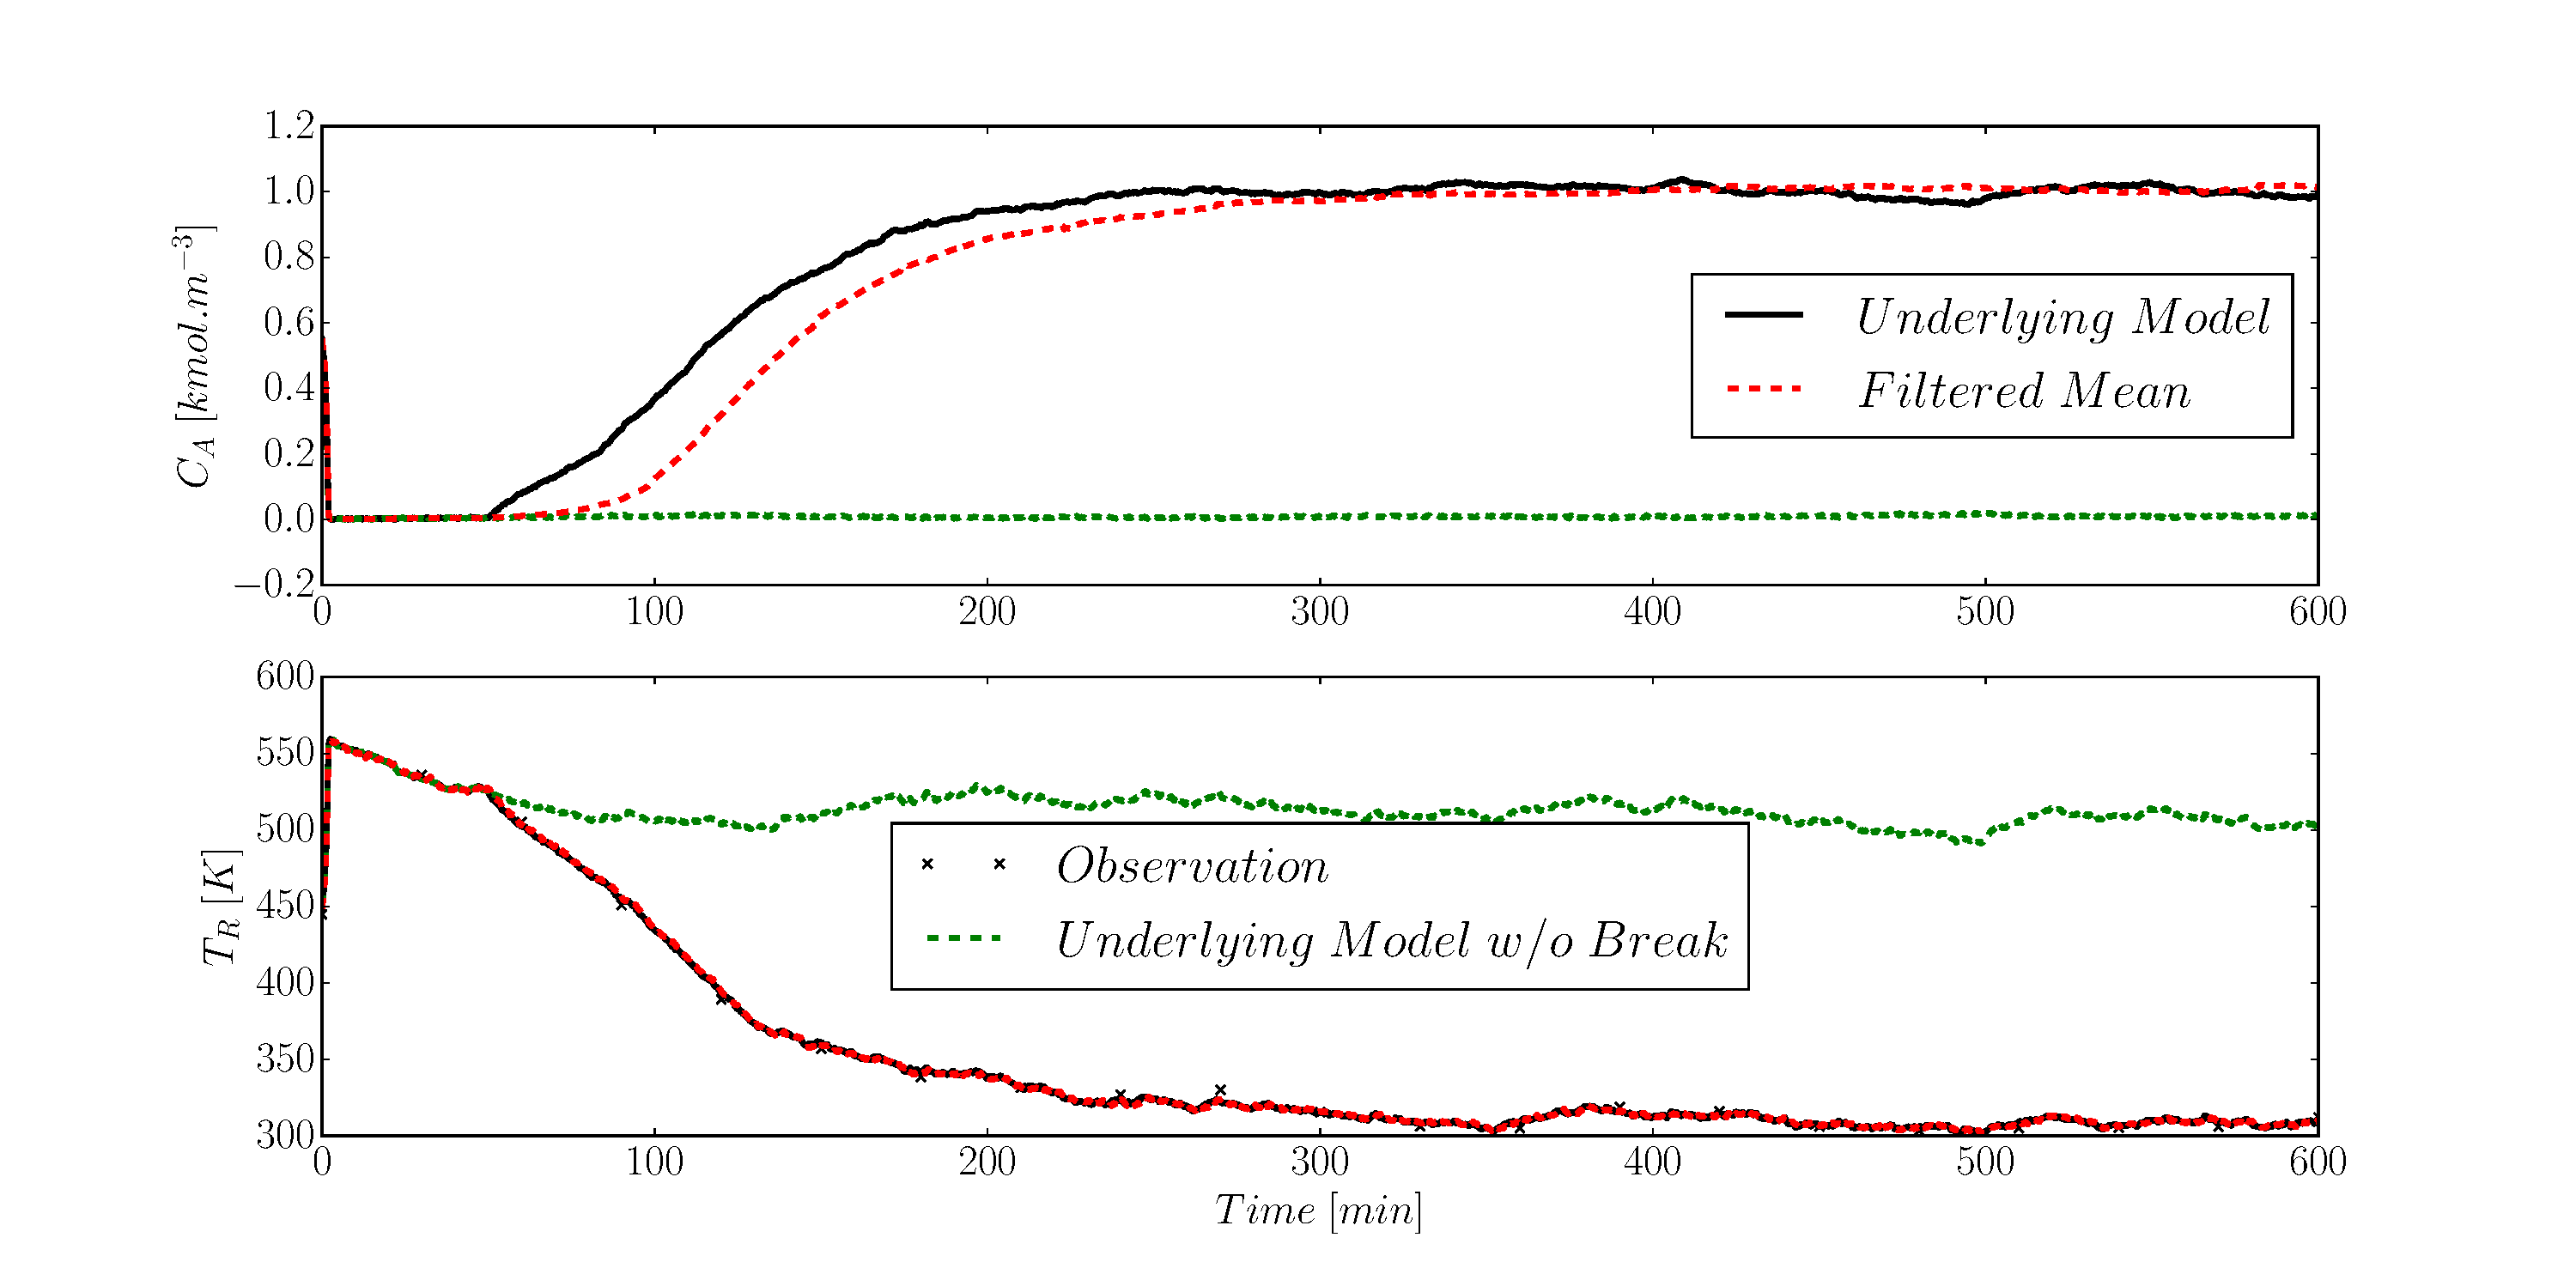
\includegraphics[width=\textwidth]{pf_m1_compspf.pdf}
\caption{Particle filter using 200 particles tracking the CSTR where the catalyst denatures at 50 minutes. Only temperature is measured.}
\label{fig_pf_m1_compspf}
\end{figure}
It is clear that the particle filter tracks the temperature well, because it is measured, but tracks the concentration very poorly. It takes almost 300 minutes before the particle filter estimates the concentration reliably. Clearly the model mismatch causes the filter's poor performance - compare this to the excellent tracking in section \ref{sec_nonlinmods_filtering}.

In figure \ref{fig_spf_m1_track} we see the tracking performance of the switching particle filter measuring only temperature.
\begin{figure}[H] 
\centering
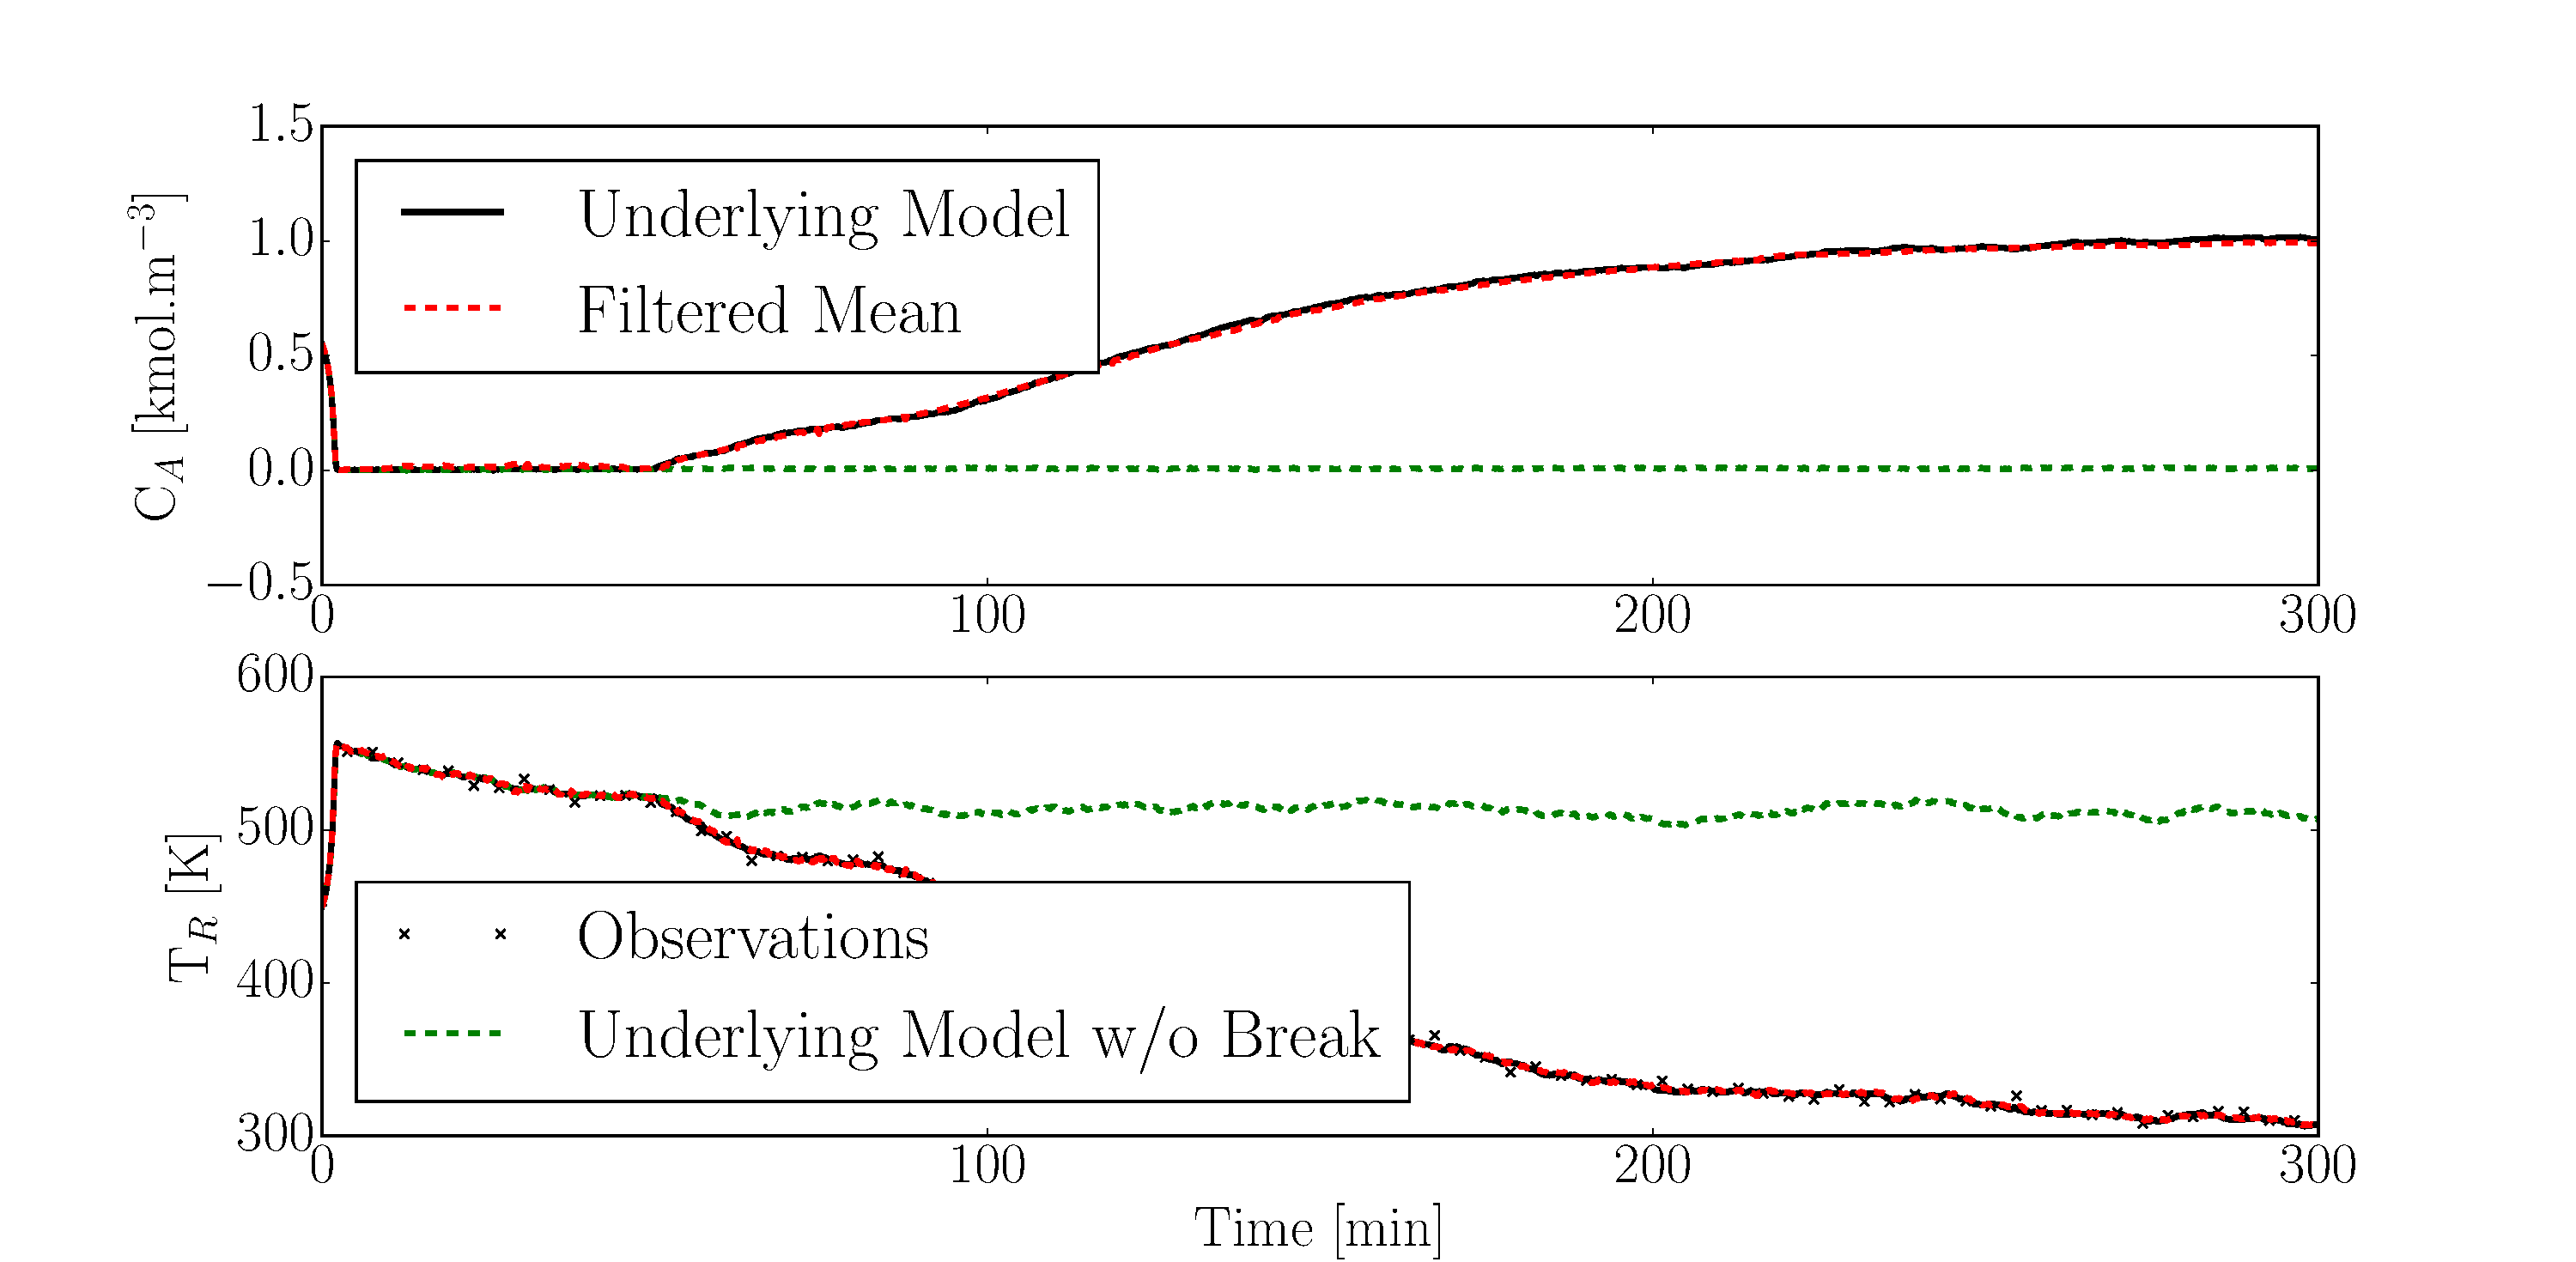
\includegraphics[width=\textwidth]{spf_m1_track.pdf}
\caption{switching particle filter using 500 particles tracking the CSTR where the catalyst denatures at 50 minutes.}
\label{fig_spf_m1_track}
\end{figure}
It is clear that the switching particle filter tracks the states very well. However, figure \ref{fig_spf_m1_switch} indicates that we have the some switching noise problems.
\begin{figure}[H] 
\centering
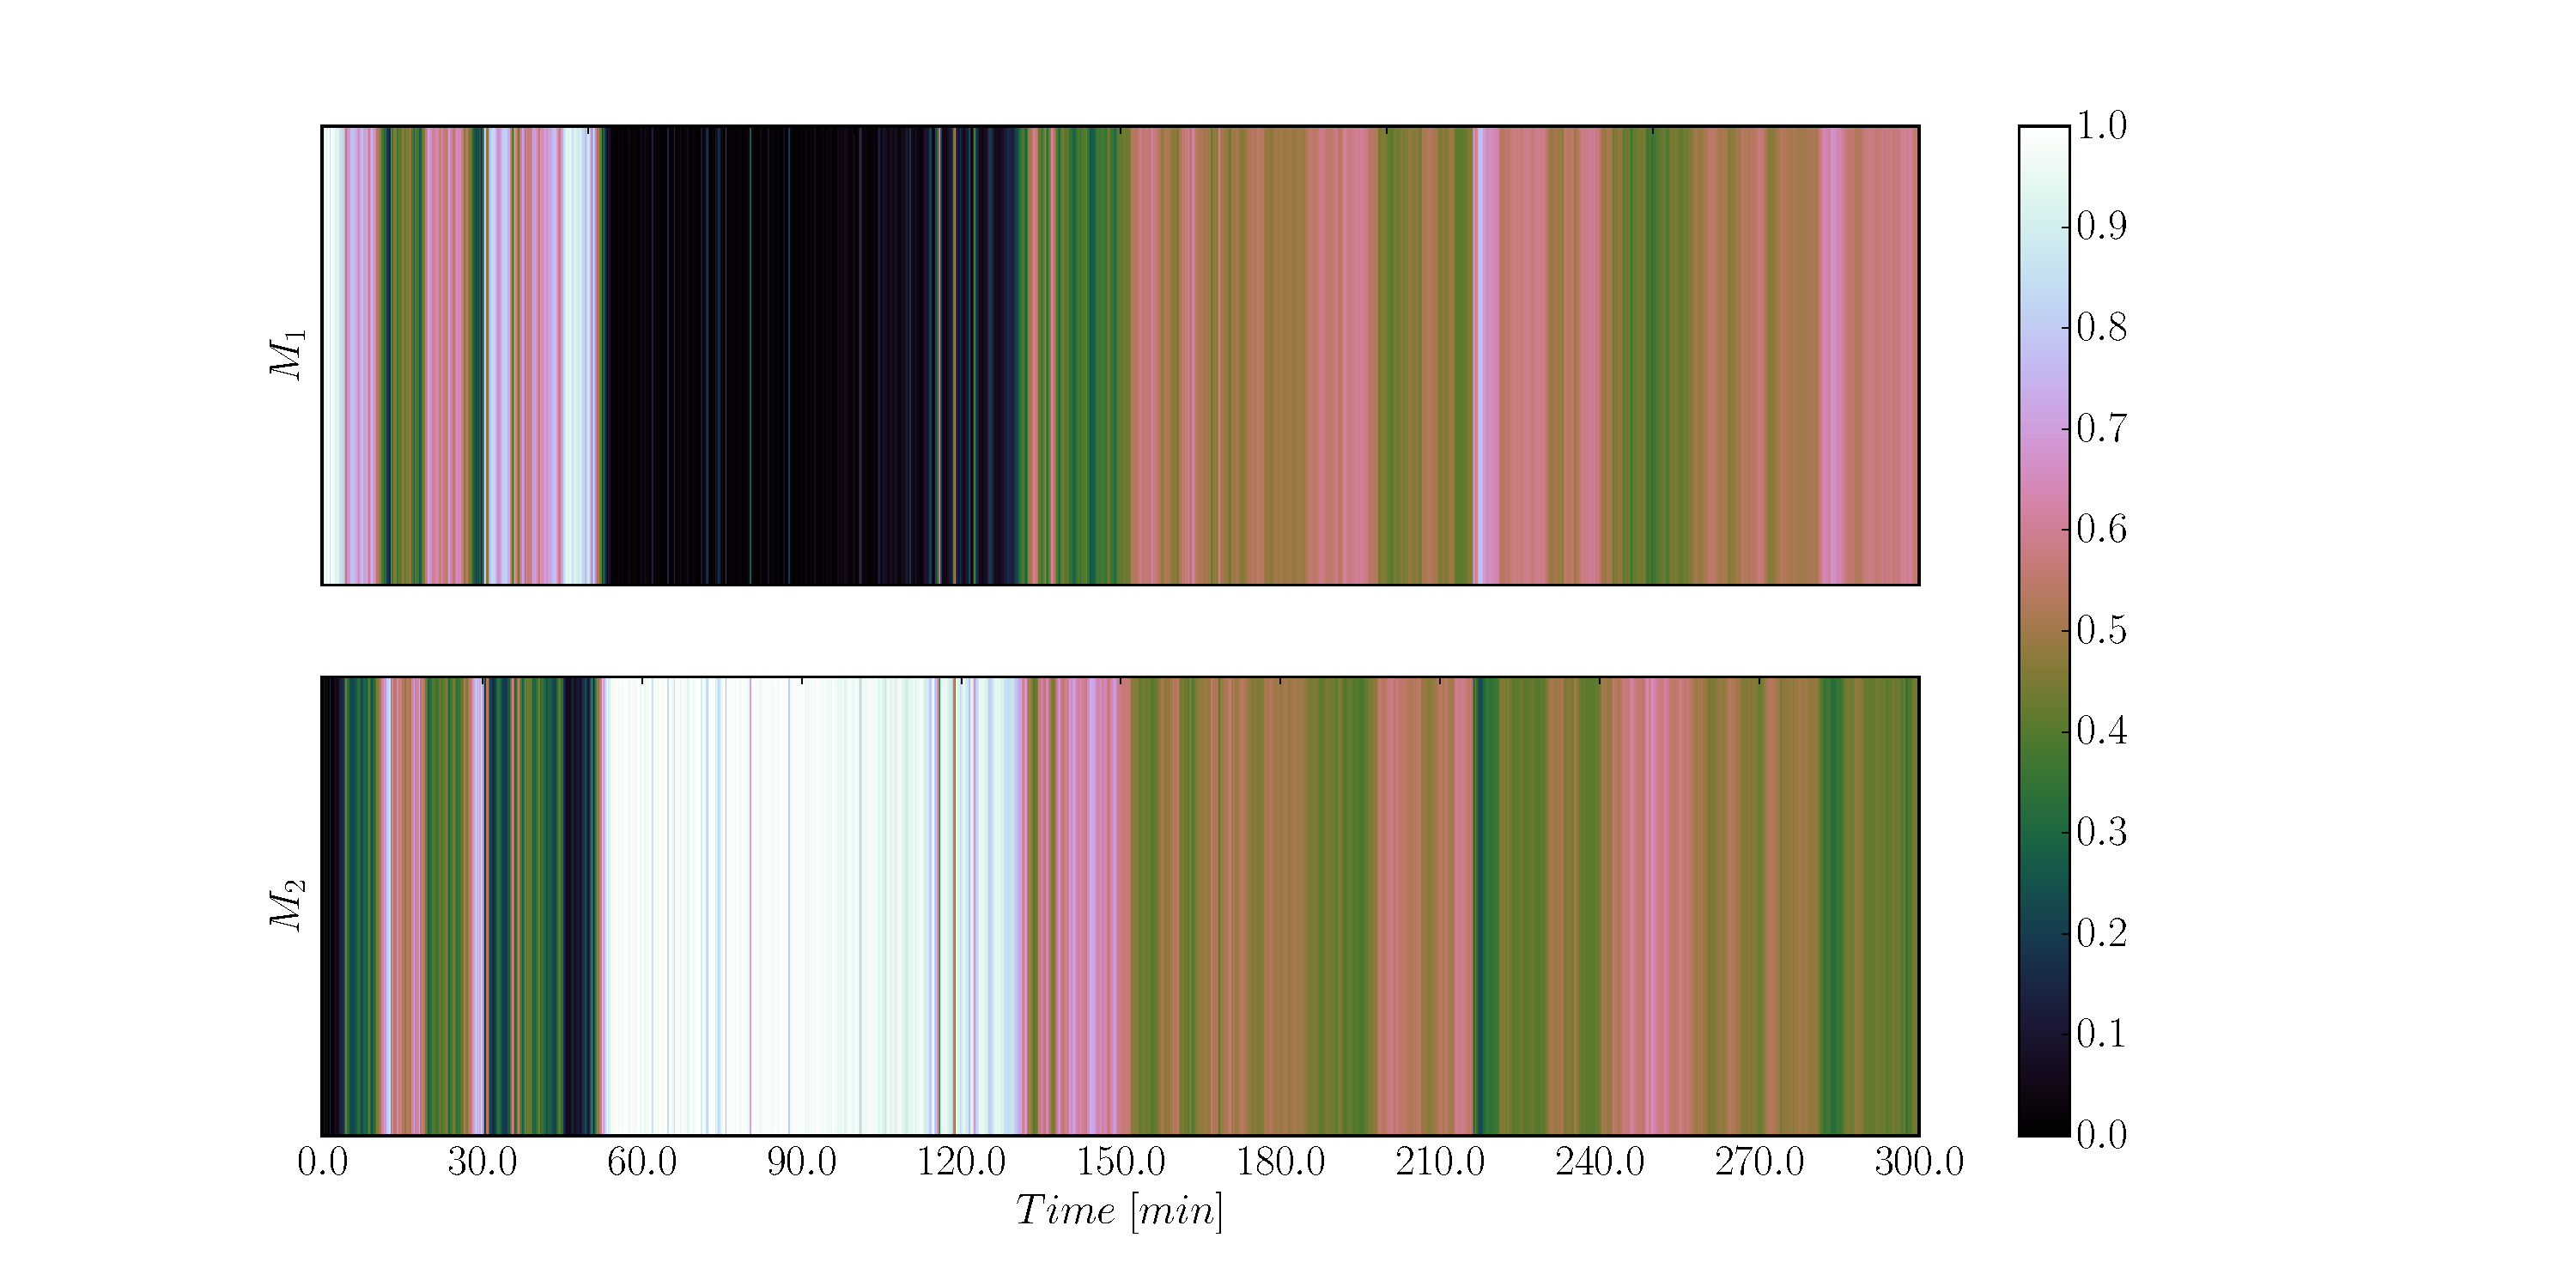
\includegraphics[width=\textwidth]{spf_m1_switch.pdf}
\caption{Switching particle filter measuring only temperature. The switching weight of each particle is shown per time step. $M_1$ corresponds to the healthy plant and $M_2$ to the broken plant.}
\label{fig_spf_m1_switch}
\end{figure} 
It is not surprising that there is switching noise: the graphical models of this and chapter \ref{sec_inf_lin_hybrid} are the same. However, we do see that the switching particle filter switches models at about 50 minutes. This indicates that the filter effectively identifies when the process fault occurs. It seems that after the fault has been identified there is a period where the filter reliably isolates the correct underlying model thereafter, from about 130 minutes, both models are equally likely. It seems there is a regime near the unstable operating point where the models are maximally different. Conversely, near the low temperature operating point (near the end of the simulation) the models are quite similar. This is physically believable because both those operating points correspond to a system where almost no conversion occurs; therefore broken or not the models would generate the similar predictions. Therefore, switching noise caused by model overlap is only a problem in this region.

Figure \ref{fig_pf_m2_compspf} illustrates the filtering performance of the particle filter using both state measurements.
\begin{figure}[H] 
\centering
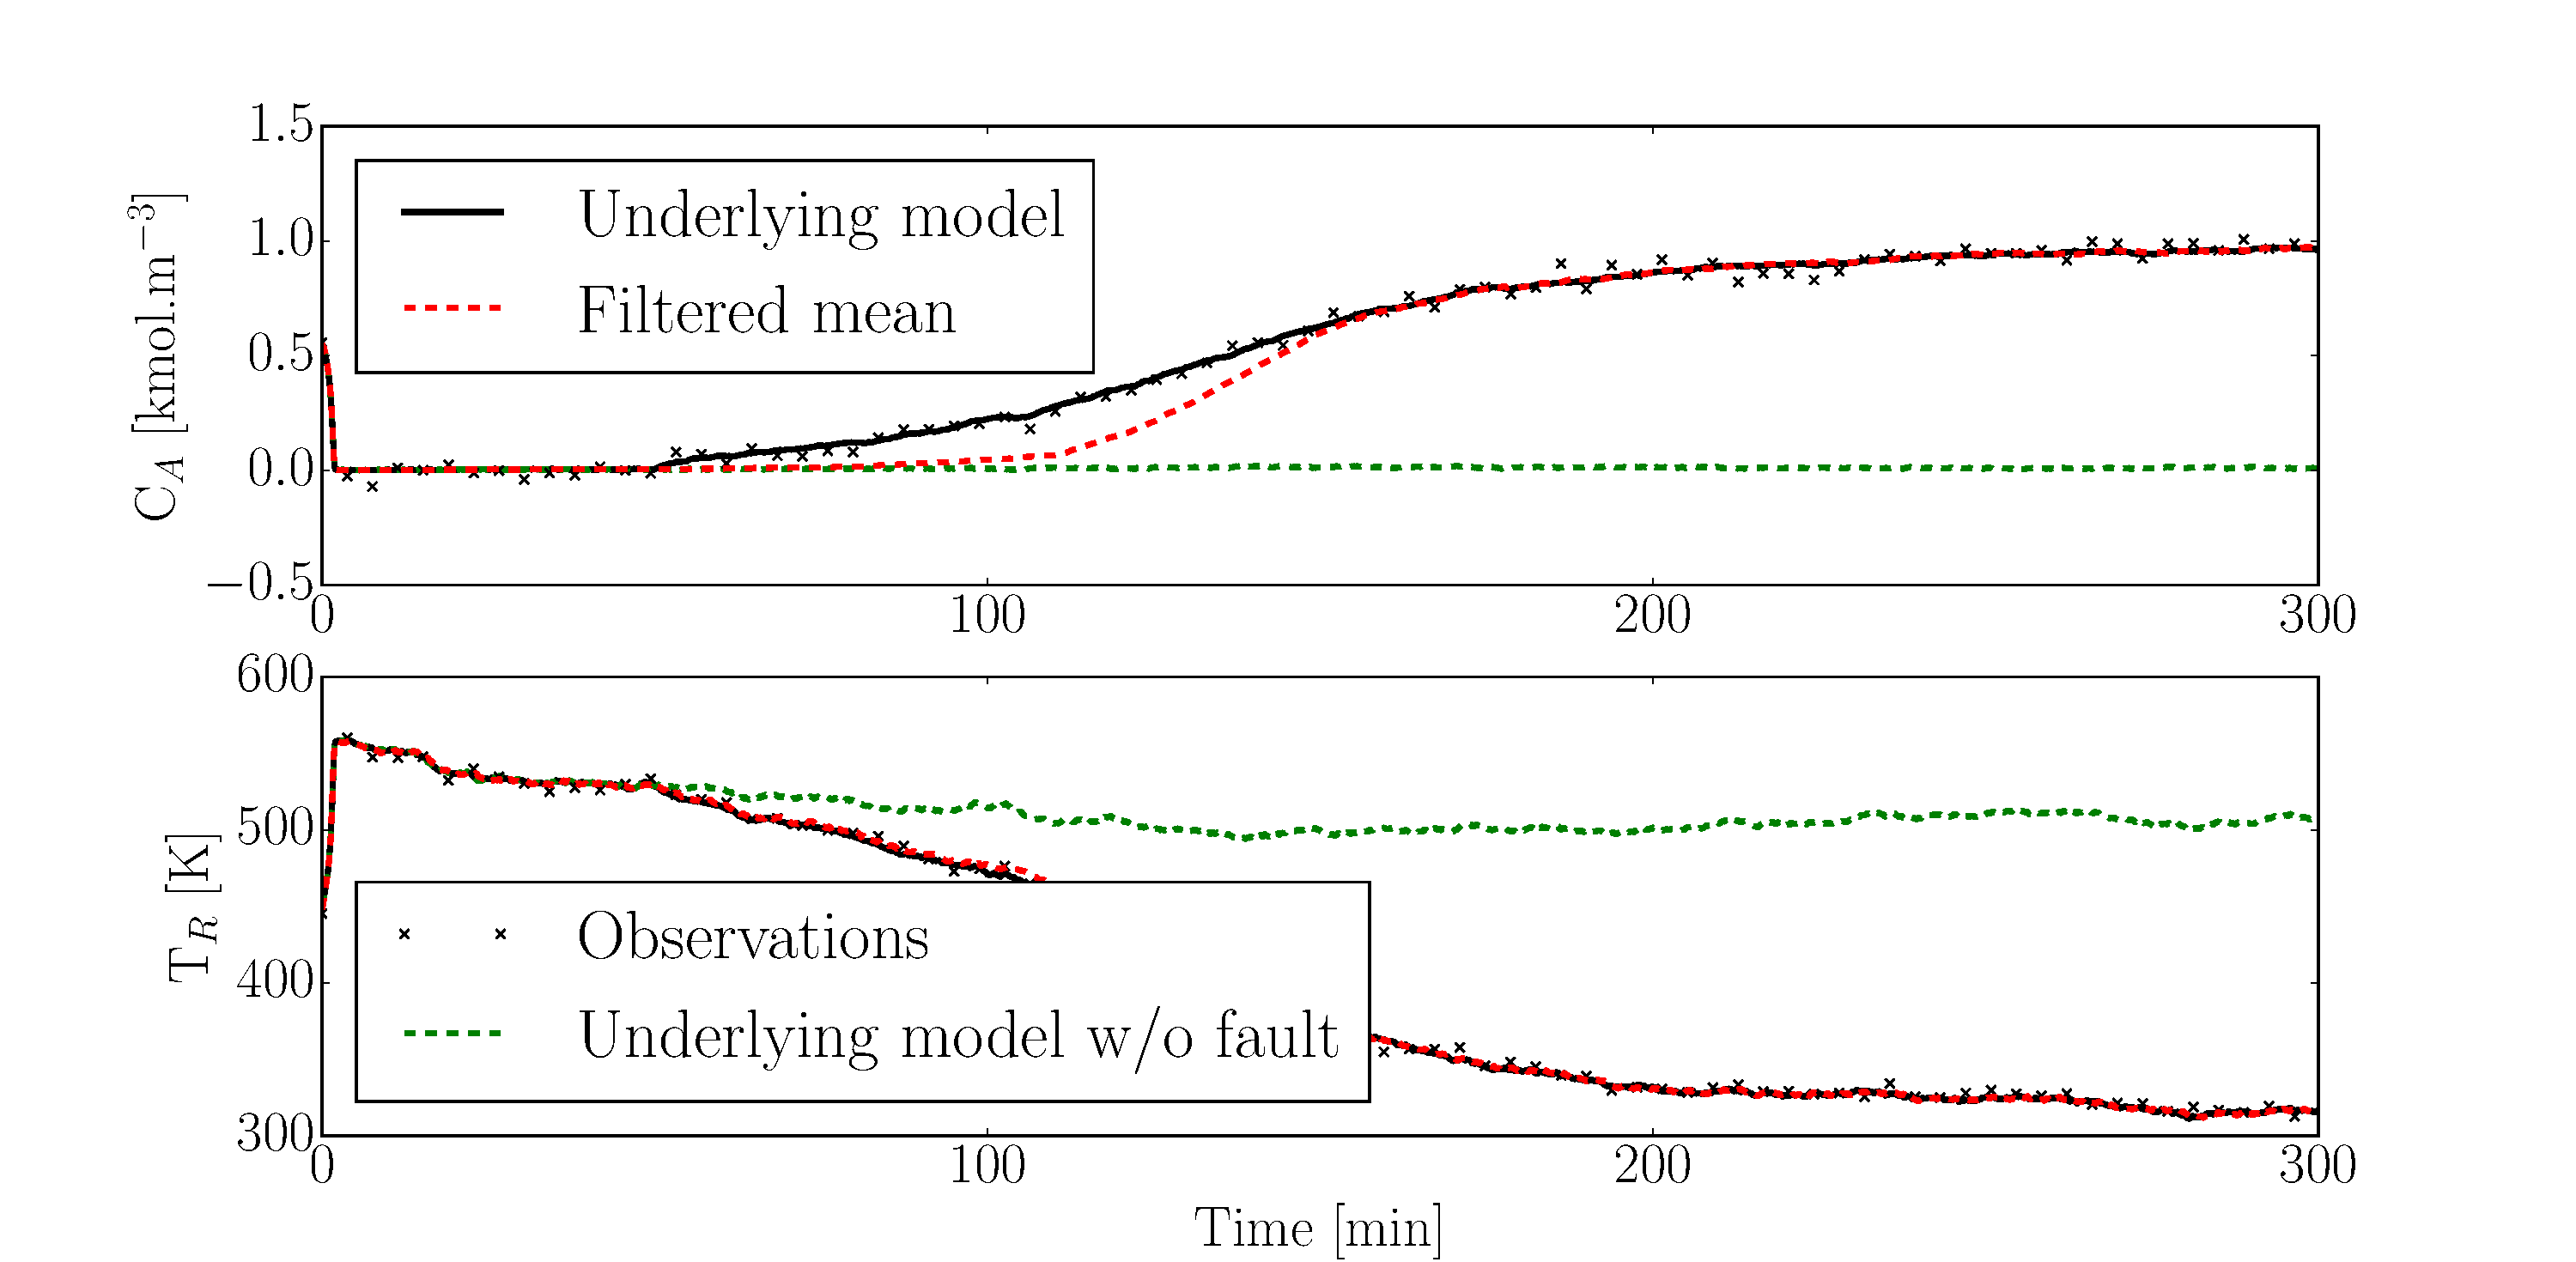
\includegraphics[width=\textwidth]{pf_m2_compspf.pdf}
\caption{Particle filter using 200 particles tracking the CSTR where the catalyst denatures at 50 minutes. Both states are measured.}
\label{fig_pf_m2_compspf}
\end{figure}
Clearly measuring both states is beneficial in terms of filter performance. The state estimation deviation seen in figure \ref{fig_pf_m1_compspf} is significantly less here - by approximately 150 minutes the particle filter is tracking the underlying system.

Figure \ref{fig_spf_m2_track} shows the filtering performance of the switching particle filter. 
\begin{figure}[H] 
\centering
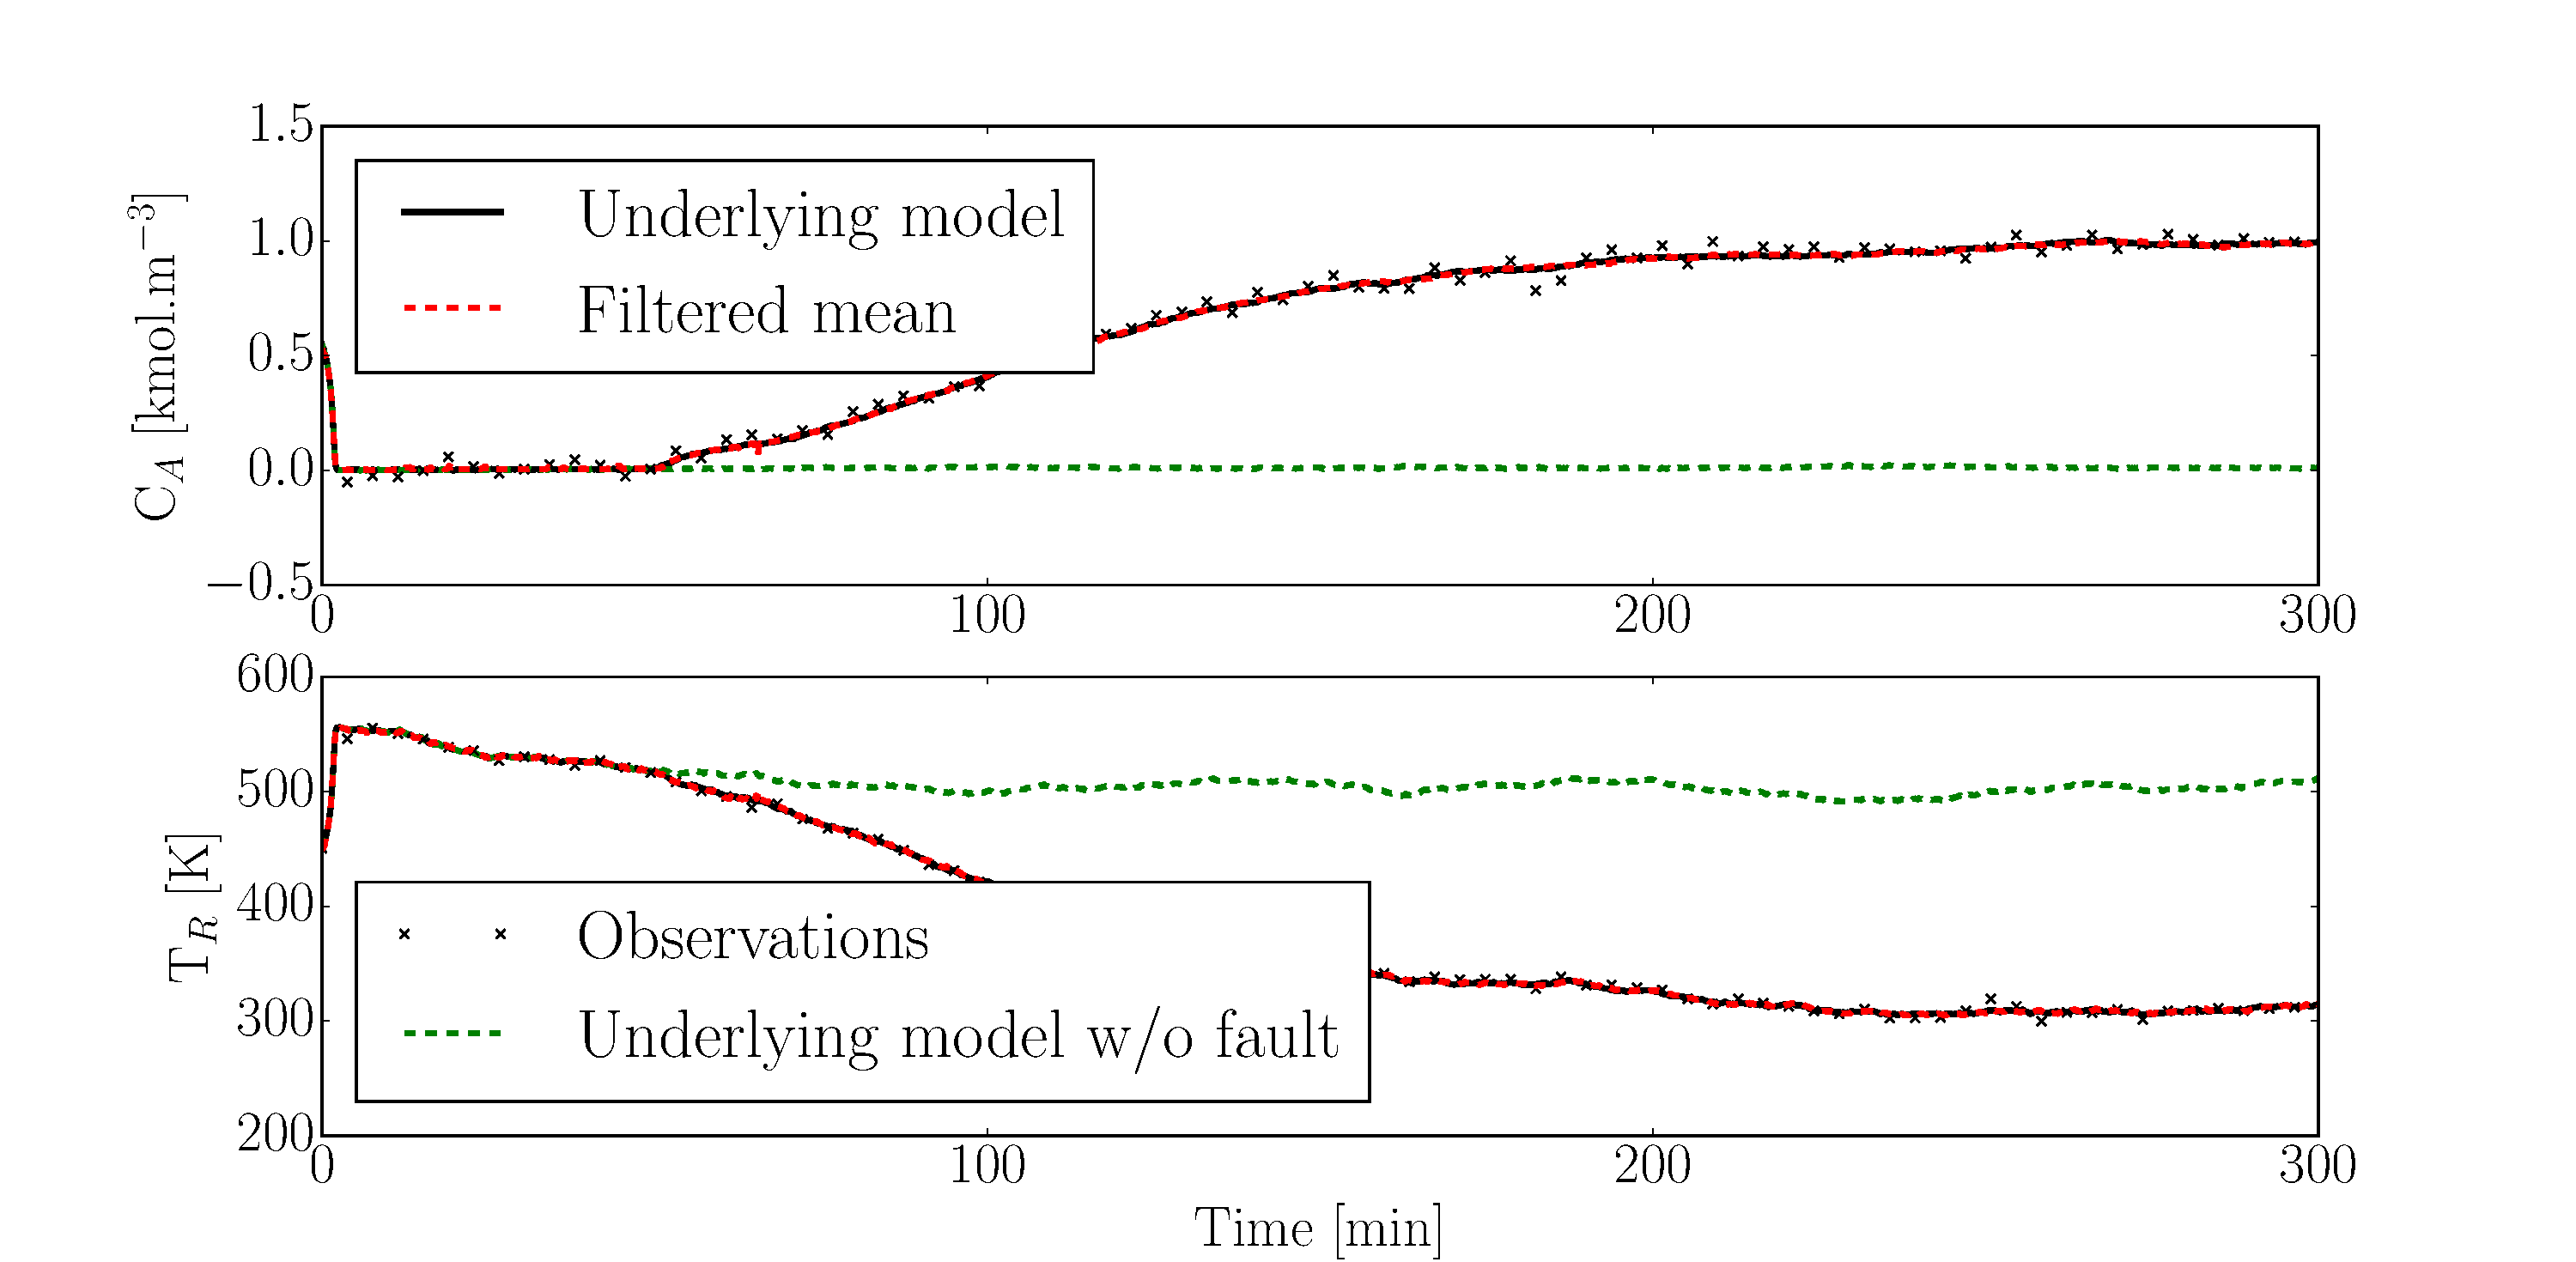
\includegraphics[width=\textwidth]{spf_m2_track.pdf}
\caption{Switching particle filter using 500 particles tracking the CSTR where the catalyst denatures at 50 minutes. Both states are measured.}
\label{fig_spf_m2_track}
\end{figure}
Again the performance is very good - the filter accurately tracks the underlying states. In figure \ref{fig_spf_m2_switch} there is significantly less switching noise in the first 100 minutes of the simulation than in figure \ref{fig_spf_m1_switch}.
\begin{figure}[H] 
\centering
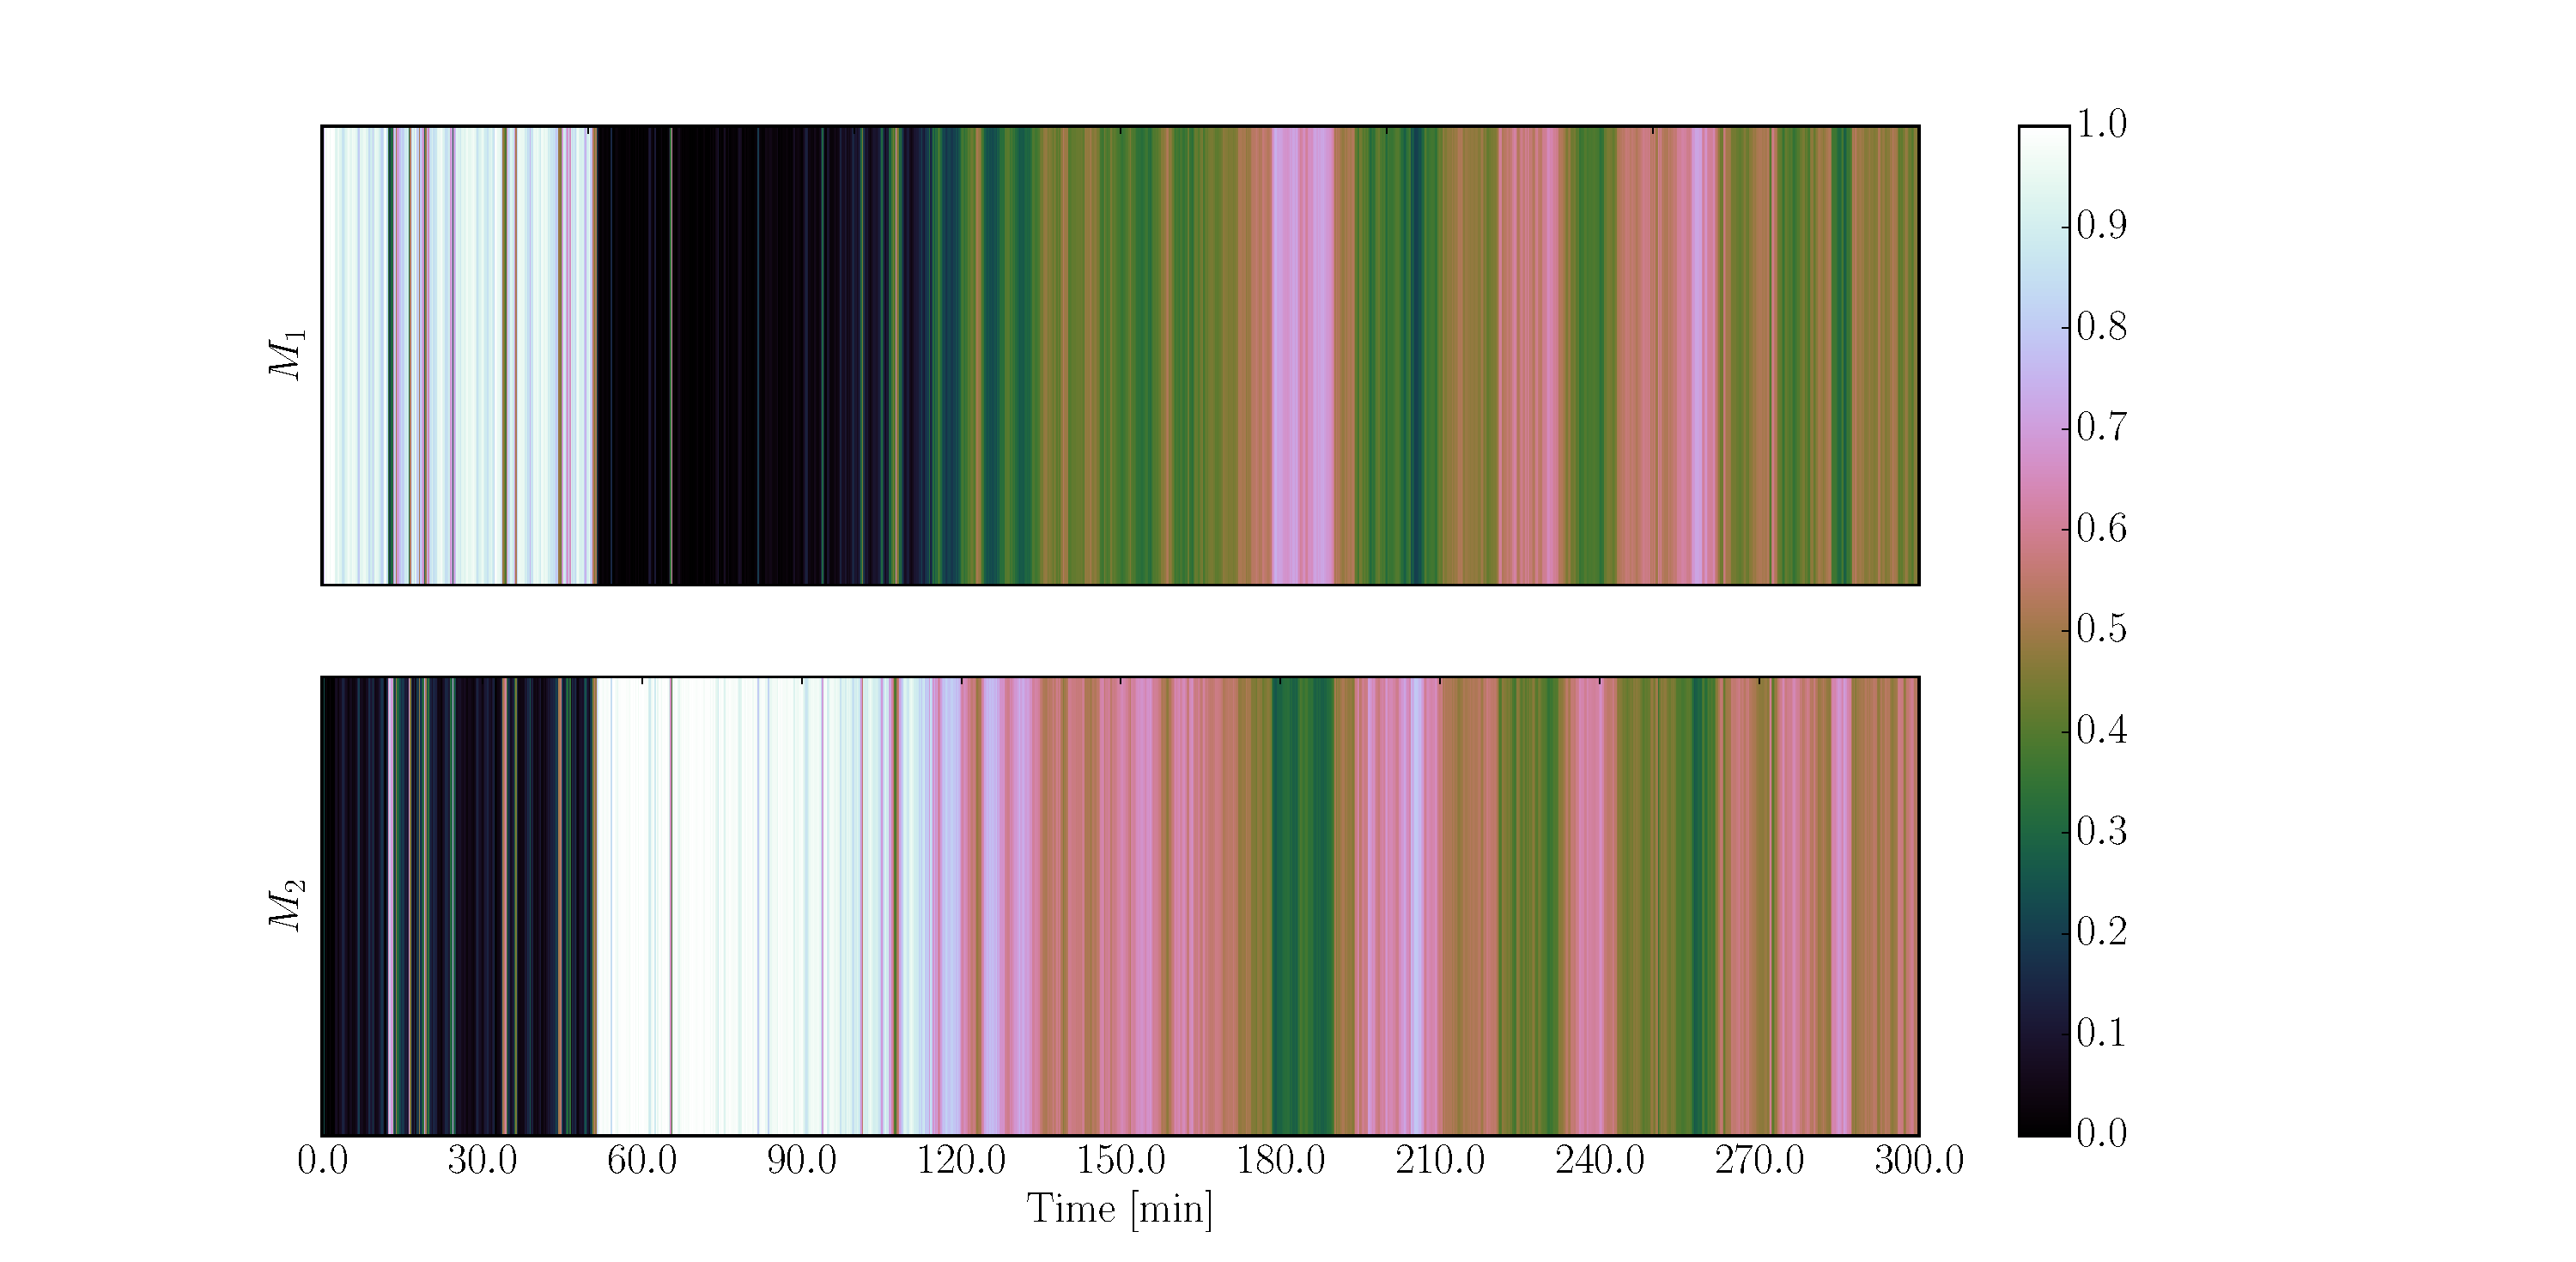
\includegraphics[width=\textwidth]{spf_m2_switch.pdf}
\caption{Switching particle filter measuring both concentration and temperature. The switching weight of each particle is shown per time step.}
\label{fig_spf_m2_switch}
\end{figure} 
It is clear that the second measurement helps the filter differentiate between the regimes of the healthy and broken plant when the system is near the high temperature and unstable operating points. However, we see the same behaviour near the low temperature operating point - the models are clearly similar here and we again have the problem of model overlap. 

In the next chapter we implement control using the switching particle filter to identify when the underlying system's dynamics have changed. 
